\documentclass[tikz,border=2pt]{standalone}
\usepackage[T1]{fontenc}
\usepackage{tgheros}
\usepackage{inconsolata}
\renewcommand{\familydefault}{\sfdefault}
\usetikzlibrary{arrows.meta,backgrounds,fit,positioning}

\definecolor{diskgreen}{HTML}{B6D7A8}
\definecolor{formatyellow}{HTML}{FFE599}
\definecolor{functionblue}{HTML}{6FA8DC}
\definecolor{memoryred}{HTML}{EA9999}

\begin{document}
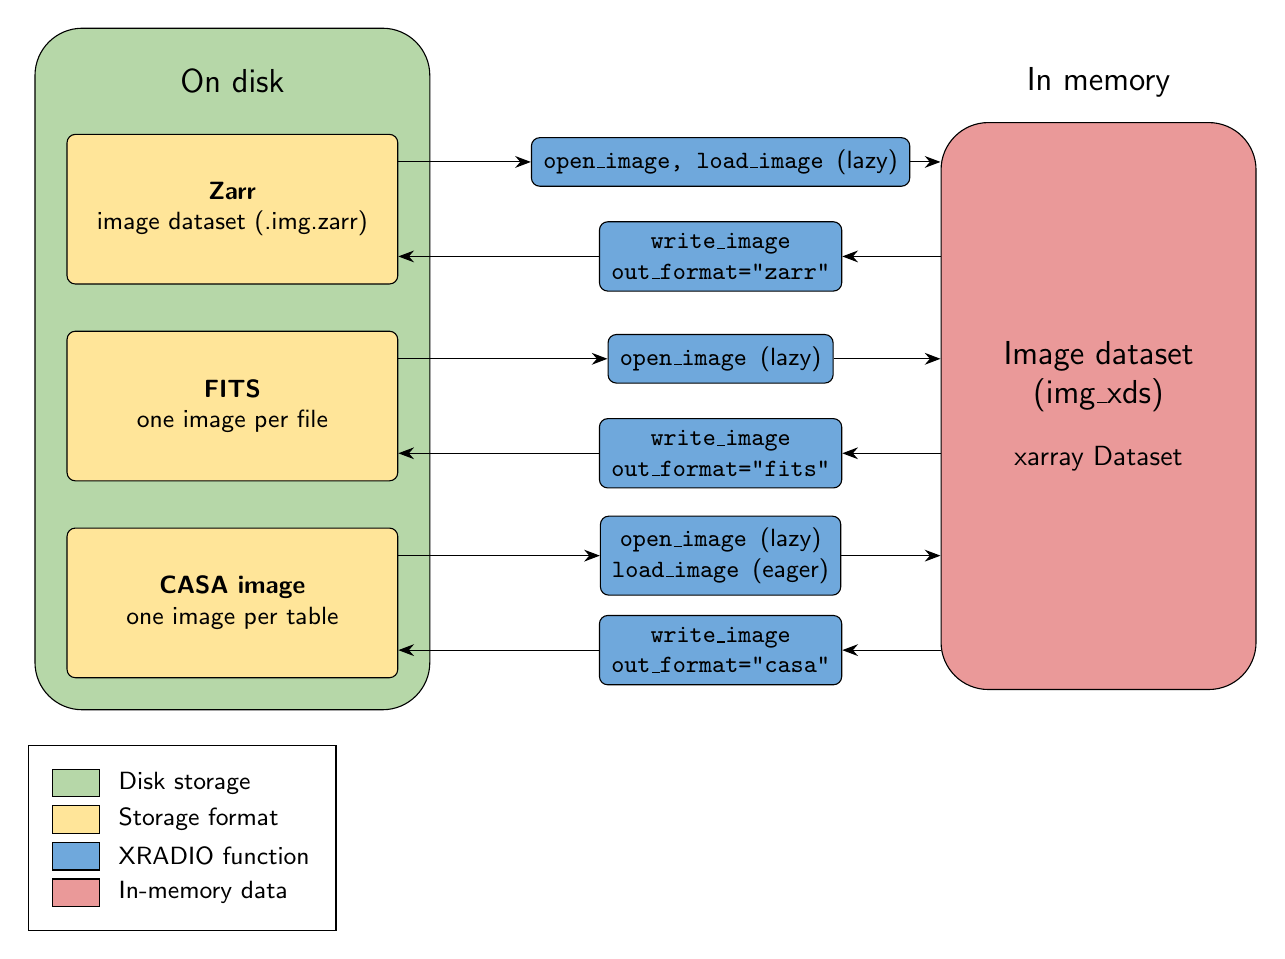
\begin{tikzpicture}[
    font=\small,
    format/.style={draw, fill=formatyellow, rounded corners=3pt,
      minimum width=4.2cm, minimum height=1.9cm, align=center},
    function/.style={draw, fill=functionblue, rounded corners=3pt,
      inner sep=1.5mm, align=center, font=\ttfamily\small},
    to/.style={-{Stealth[length=2mm]}},
    title/.style={font=\large},
  ]
  \node[format] (zarr) at (0, 5) {\textbf{Zarr}\\ image dataset (.img.zarr)};
  \node[format] (fits) at (0, 2.5) {\textbf{FITS}\\ one image per file};
  \node[format] (casa) at (0, 0) {\textbf{CASA image}\\ one image per table};

  \node[draw, fill=memoryred, rounded corners=6mm, minimum width=4cm,
    minimum height=7.2cm, align=center, font=\large] (img) at (11, 2.5)
    {Image dataset\\ (img\_xds)\\[3mm] \normalsize xarray Dataset};

  \foreach \f/\read/\out in {
      zarr/{open\_image, load\_image \textsf{(lazy)}}/zarr,
      fits/{open\_image \textsf{(lazy)}}/fits,
      casa/{open\_image \textsf{(lazy)}\\ load\_image \textsf{(eager)}}/casa} {
    \node[function] (read \f) at ([yshift=6mm]6.2, 0 |- \f) {\read};
    \node[function] (write \f) at ([yshift=-6mm]6.2, 0 |- \f)
      {write\_image\\ out\_format="\out"};
    \draw[to] (\f.east |- read \f) -- (read \f);
    \draw[to] (read \f) -- (img.west |- read \f);
    \draw[to] (img.west |- write \f) -- (write \f);
    \draw[to] (write \f) -- (\f.east |- write \f);
  }

  \node[title, above=4mm of zarr] (disk title) {On disk};
  \node[title, above=2mm of img] {In memory};
  \begin{scope}[on background layer]
    \node[draw, rounded corners=6mm, inner sep=4mm, fill=diskgreen,
      fit=(disk title) (zarr) (casa)] {};
  \end{scope}

  \matrix[draw, anchor=north west, column sep=2mm, row sep=1mm, inner sep=3mm,
      nodes={anchor=west, inner sep=1pt}] at (-2.6, -1.8) {
    \node[draw, fill=diskgreen, minimum width=6mm, minimum height=3.5mm] {}; &
      \node {Disk storage}; \\
    \node[draw, fill=formatyellow, minimum width=6mm, minimum height=3.5mm] {}; &
      \node {Storage format}; \\
    \node[draw, fill=functionblue, minimum width=6mm, minimum height=3.5mm] {}; &
      \node {XRADIO function}; \\
    \node[draw, fill=memoryred, minimum width=6mm, minimum height=3.5mm] {}; &
      \node {In-memory data}; \\
  };
\end{tikzpicture}
\end{document}
